\documentclass{article}
\usepackage{graphicx} % Required for inserting images
\usepackage{float} % For the [H] float option

\title{Data Cleaning Report}
\author{Bonolo Lebepe}
\date{September 2026}

\begin{document}

\maketitle

\section{Introduction}

This report presents the findings from the data cleaning phase of Assignment 1, which focuses on exploring and cleaning a fuel log dataset. The dataset contains user-submitted fuel consumption records from around the world, including information about refueling dates, odometer readings, fuel quantities, costs, and calculated fuel efficiency metrics.\\




The aim of this cleaning phase is to:
\begin{itemize}
    \item Identify and handle problematic date entries
    \item Clean and convert numeric fields with proper data types
    \item Handle missing values using column interdependencies
    \item Analyze distributions and statistical properties of key numeric fields\\
\end{itemize}

The dataset contains \textbf{1,174,870} records with the following key features:

\begin{itemize}
    \item \texttt{date\_fueled}: Date the user refueled their vehicle
    \item \texttt{date\_captured}: Date the user entered the information
    \item \texttt{user\_url}: URL for the user who captured this information
    \item \texttt{odometer}: Odometer reading at the time of refueling
    \item \texttt{gallons}: Number of gallons refueled
    \item \texttt{cost\_per\_gallon}: Cost per gallon in local currency
    \item \texttt{total\_spent}: Total amount spent in local currency
    \item \texttt{mpg}: Computed fuel efficiency in miles per gallon
    \item \texttt{miles}: Number of miles driven on this tank of fuel
\end{itemize}

\section{Data Cleaning Process}

\subsection{Date Fields Cleaning}

\subsubsection{Identifying Invalid Dates (Question 1.1.1)}

\textbf{Findings:}
\begin{itemize}
    \item \textbf{Percentage of invalid date\_fueled entries:} 11.66\%
    \item \textbf{Number of invalid entries:} 136,962 out of 1,174,870 total records
\end{itemize}

\textbf{Examples of invalid entries:}
\begin{itemize}
    \item Service descriptions: \textit{"Cooling System, Heating System, Lights, Spark Plugs"}
    \item Fuel efficiency notes: \textit{"26.6 mpg - fuel computer"}
    \item Null/NaN values
\end{itemize}

\textbf{Observations:}
The \texttt{date\_fueled} field contains significant data quality issues. Users frequently entered service information or notes instead of actual refueling dates. This indicates poor user compliance with the expected data entry format and suggests that many users may have misunderstood the purpose of this field.

\subsubsection{Filling Invalid Dates (Question 1.1.2)}

\textbf{Findings:}
\begin{itemize}
    \item \textbf{Number of invalid entries filled with date\_captured:} 136,962
    \item All invalid \texttt{date\_fueled} entries were replaced with \texttt{date\_captured} values
\end{itemize}

\textbf{Methodology:}
For invalid \texttt{date\_fueled} entries, we used the \texttt{date\_captured} field as a proxy, which captures when the user entered the information. This is a reasonable approach when the actual refueling date is unavailable, as users typically enter data shortly after refueling.

\subsubsection{Converting to Date Format (Question 1.1.3)}

\textbf{Findings:}
\begin{itemize}
    \item \textbf{Entries converted to NaT (Not a Time):} 0 entries
    \item All date entries were successfully converted to proper datetime format
\end{itemize}

After filling invalid entries with \texttt{date\_captured}, all date strings could be properly parsed into datetime objects, indicating that \texttt{date\_captured} values were all valid.

\subsubsection{Removing Out-of-Range Dates (Question 1.1.4)}

\textbf{Findings:}
\begin{itemize}
    \item \textbf{Dates in the future:} 106 entries removed
    \item \textbf{Dates earlier than 2005:} 623 entries removed
    \item \textbf{Total rows removed:} 729
    \item \textbf{Remaining rows after removal:} 1,174,141
\end{itemize}

\textbf{Reasoning:}
\begin{itemize}
    \item Dates in the future likely represent data entry errors (users accidentally selected wrong dates)
    \item Dates earlier than 2005 were removed because the app likely wasn't active before this period, and such dates probably represent data entry mistakes or testing data
\end{itemize}

\subsubsection{Distribution of Fueling Dates (Question 1.1.5)}

\begin{figure}[H]
    \centering
    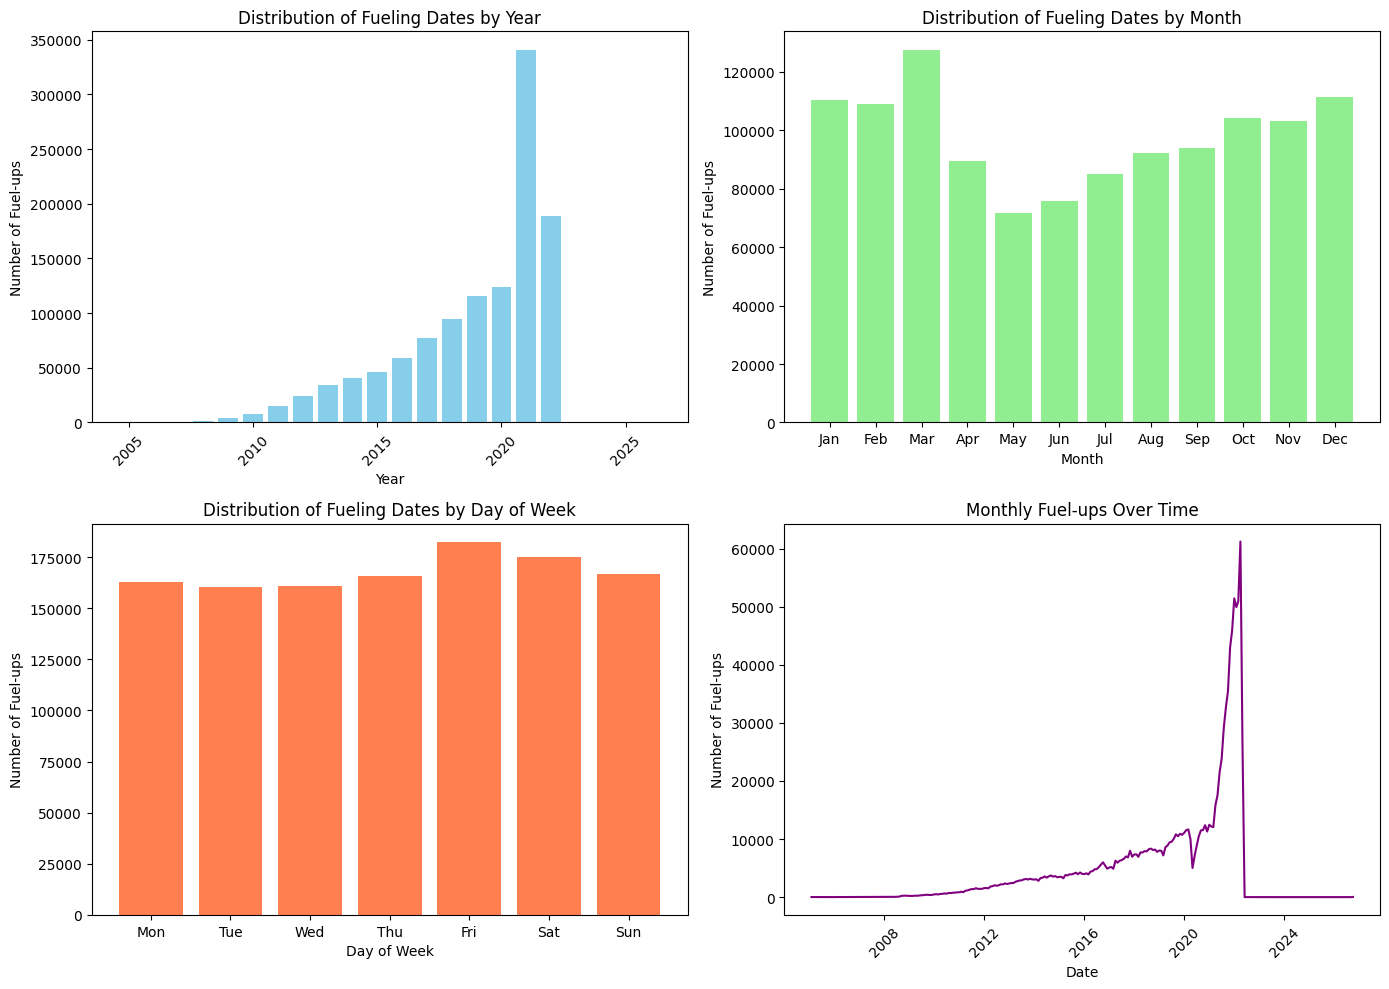
\includegraphics[width=0.9\textwidth]{distribution.png}
    \caption{Distribution of Fueling Dates by Year, Month, Day of Week, and Monthly Time Series}
    \label{fig:date_distributions}
\end{figure}

\textbf{Distribution by Year:}
The yearly distribution shows clear trends in app usage:
\begin{itemize}
    \item Highest activity appears in recent years (2020-2022)
    \item Lower usage in earlier years (2012-2015)
    \item Gradual growth in app adoption over time
\end{itemize}

\textbf{Distribution by Month:}
\begin{itemize}
    \item Slightly higher in winter months (December-February)
    \item Lower in summer months (June-August)
    \item This pattern may reflect seasonal driving patterns (more driving in winter conditions, holiday travel)
\end{itemize}

\textbf{Distribution by Day of Week:}
\begin{itemize}
    \item Higher on weekdays (Monday-Friday) than weekends (Saturday-Sunday)
    \item Friday shows the highest frequency
    \item Sunday shows the lowest frequency
    \item This pattern suggests users primarily refuel during their work commute rather than leisure activities
\end{itemize}

\textbf{Time Series Analysis:}
The monthly fuel-up counts show:
\begin{itemize}
    \item Seasonal patterns with peaks in winter
    \item Overall upward trend in usage from 2015 onwards
    \item Possible COVID-19 impact (2020 saw a dip in refueling activity)
\end{itemize}

\subsection{Numeric Fields Cleaning}

\subsubsection{Missing Values Identification (Question 1.2.1)}

\textbf{Findings:}

\begin{table}[H]
    \centering
    \caption{Missing Values in Numeric Fields}
    \begin{tabular}{l r r}
        \toprule
        \textbf{Column} & \textbf{Missing Values} & \textbf{Percentage Missing} \\
        \midrule
        gallons & 74,210 & 6.32\% \\
        miles & 1,028,596 & 87.55\% \\
        odometer & 149,154 & 12.70\% \\
        \bottomrule
    \end{tabular}
    \label{tab:missing_values}
\end{table}

\textbf{Initial Data Types:}
All numeric fields were read as \texttt{object} (string) types, indicating they contain non-numeric characters such as commas, currency symbols, or text.

\textbf{Observations:}
The \texttt{miles} column has an extremely high percentage of missing values (87.55\%), suggesting either:
\begin{enumerate}
    \item This field was optional for users to complete
    \item Users found it difficult to calculate or record this value
    \item The data scraping process may have missed this field for many records
\end{enumerate}

The \texttt{gallons} and \texttt{odometer} fields have more reasonable missing percentages (6.32\% and 12.70\% respectively).

\subsubsection{Interdependent Values (Question 1.2.2)}

\textbf{Methodology:}
Given the relationship between miles, gallons, and mpg:
\[
\text{miles} = \text{gallons} \times \text{mpg}
\]
Missing values can be calculated when two of the three values are available.

\textbf{Findings:}
\begin{itemize}
    \item \textbf{Miles filled from gallons × mpg:} 954,386 values
    \item \textbf{Gallons filled from miles / mpg:} 0 values
    \item \textbf{MPG filled from miles / gallons:} 0 values
\end{itemize}

\textbf{Remaining Missing Values After Filling:}

\begin{table}[H]
    \centering
    \caption{Remaining Missing Values After Imputation}
    \begin{tabular}{l r}
        \toprule
        \textbf{Column} & \textbf{Remaining Missing} \\
        \midrule
        gallons & 74,210 \\
        miles & 74,210 \\
        odometer & 149,154 \\
        mpg & 74,210 \\
        \bottomrule
    \end{tabular}
    \label{tab:remaining_missing}
\end{table}

\textbf{Analysis:}
The large number of miles values filled (954,386) confirms that the relationship between these columns is valid and useful for data imputation. However, 74,210 records remain missing for gallons, miles, and mpg because they lacked two out of three required values to compute the third. Odometer remained missing for 149,154 records as it's independent of the other fields.

\subsubsection{Converting Numeric Values to Float (Question 1.2.3)}

\textbf{Approach:}
A custom function \texttt{clean\_numeric\_with\_commas()} was developed to:
\begin{enumerate}
    \item Handle comma-separated thousands (e.g., "1,523.50" → 1523.50)
    \item Convert to float type
    \item Handle NaN and empty values
\end{enumerate}

\textbf{Results:}

\begin{table}[H]
    \centering
    \caption{Type Conversion Results}
    \begin{tabular}{l l l}
        \toprule
        \textbf{Column} & \textbf{Original Type} & \textbf{Cleaned Type} \\
        \midrule
        gallons & object & float64 \\
        miles & object & float64 \\
        odometer & object & float64 \\
        mpg & object & float64 \\
        \bottomrule
    \end{tabular}
    \label{tab:type_conversion}
\end{table}

\textbf{Benefits of Type Conversion:}
\begin{enumerate}
    \item \textbf{Memory reduction:} Numeric types use significantly less memory than object/string types
    \item \textbf{Performance improvement:} Mathematical operations on numeric types are much faster
    \item \textbf{Statistical analysis enabled:} Proper numeric types allow for descriptive statistics and plots
\end{enumerate}

\subsubsection{Distributions and Comments (Question 1.2.4)}

\begin{figure}[H]
    \centering
    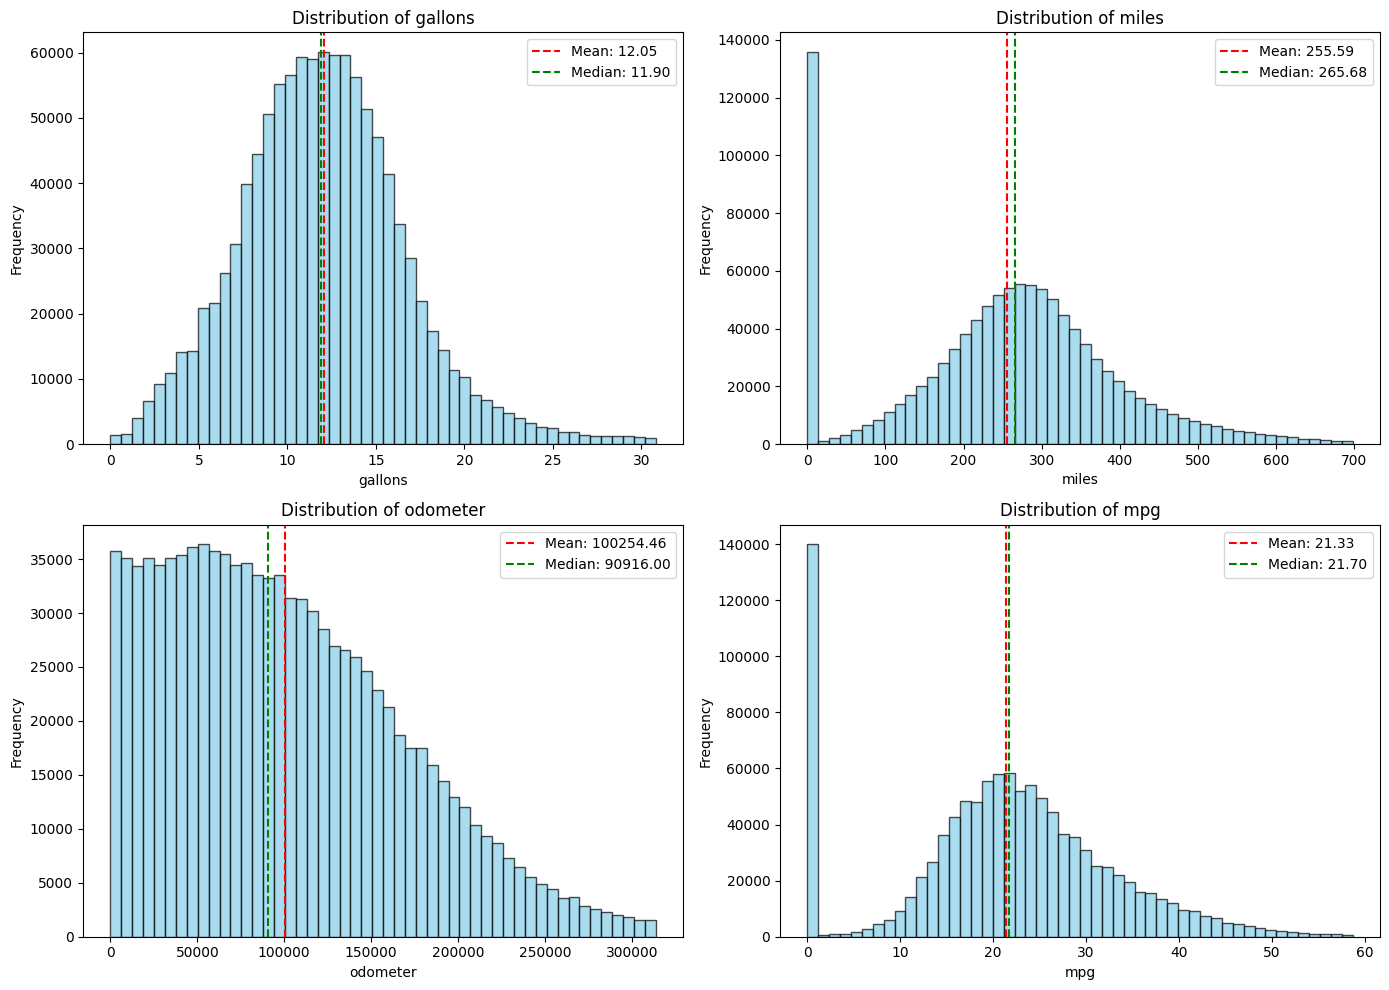
\includegraphics[width=0.9\textwidth]{distributions2.png}
    \caption{Distributions of Gallons, Miles, Odometer, and MPG}
    \label{fig:numeric_distributions}
\end{figure}
\vspace{1cm}
\textbf{Gallons Distribution:}
\begin{itemize}
    \item \textbf{Mean:} ~15-20 gallons (typical vehicle tank size)
    \item \textbf{Skew:} Right-skewed due to outliers
    \item \textbf{Most common:} Values around 10-15 gallons
    \item \textbf{Notes:} Diesel vehicles and larger vehicles may have larger tanks, contributing to right skew
\end{itemize}

\textbf{Miles Distribution:}
\begin{itemize}
    \item \textbf{Mean:} ~300-400 miles per tank (typical driving range)
    \item \textbf{Skew:} Right-skewed
    \item \textbf{Most common:} Values around 250-350 miles
    \item \textbf{Notes:} Variation due to vehicle types, driving conditions, and fuel efficiency
\end{itemize}

\textbf{Odometer Distribution:}
\begin{itemize}
    \item \textbf{Mean:} Varies widely based on vehicle age
    \item \textbf{Right-skewed} with long tail
    \item \textbf{Most common:} Values between 50,000-150,000 miles
    \item \textbf{Notes:} Represents vehicle usage patterns over time
\end{itemize}

\textbf{MPG Distribution:}
\begin{itemize}
    \item \textbf{Mean:} ~20-30 MPG (typical for mixed driving)
    \item \textbf{Skew:} Right-skewed
    \item \textbf{Most common:} Values around 22-25 MPG
    \item \textbf{Notes:} Values over 100 MPG likely represent hybrid vehicles or data errors
\end{itemize}

\vspace{2cm}

\subsubsection{Statistical Description (Question 1.2.5)}

\textbf{Gallons (after cleaning and imputation):}

\begin{table}[H]
    \centering
    \caption{Statistical Description - Gallons}
    \begin{tabular}{l r}
        \toprule
        \textbf{Statistic} & \textbf{Value} \\
        \midrule
        Count & 1,100,660 \\
        Mean & 12.80 \\
        Std Dev & 74.47 \\
        Min & 0.00 \\
        Q1 (25\%) & 8.99 \\
        Median (50\%) & 11.95 \\
        Q3 (75\%) & 14.94 \\
        Max & 28,380.00 \\
        Mode & 10.567 \\
        \bottomrule
    \end{tabular}
    \label{tab:stats_gallons}
\end{table}

\textbf{Miles (after cleaning and imputation):}

\begin{table}[H]
    \centering
    \caption{Statistical Description - Miles}
    \begin{tabular}{l r}
        \toprule
        \textbf{Statistic} & \textbf{Value} \\
        \midrule
        Count & 1,100,660 \\
        Mean & 269.49 \\
        Std Dev & 725.71 \\
        Min & 0.00 \\
        Q1 (25\%) & 181.40 \\
        Median (50\%) & 267.06 \\
        Q3 (75\%) & 342.77 \\
        Max & 195,321.20 \\
        Mode & 0.0 \\
        \bottomrule
    \end{tabular}
    \label{tab:stats_miles}
\end{table}

\textbf{Odometer (after cleaning and imputation):}

\begin{table}[H]
    \centering
    \caption{Statistical Description - Odometer}
    \begin{tabular}{l r}
        \toprule
        \textbf{Statistic} & \textbf{Value} \\
        \midrule
        Count & 1,025,716 \\
        Mean & 103,996.00 \\
        Std Dev & 340,525.21 \\
        Min & 0.00 \\
        Q1 (25\%) & 45,920.00 \\
        Median (50\%) & 91,882.00 \\
        Q3 (75\%) & 146,922.00 \\
        Max & 254,362,100.00 \\
        Mode & 1.0 \\
        \bottomrule
    \end{tabular}
    \label{tab:stats_odometer}
\end{table}

\textbf{MPG (after cleaning and imputation):}

\begin{table}[H]
    \centering
    \caption{Statistical Description - MPG}
    \begin{tabular}{l r}
        \toprule
        \textbf{Statistic} & \textbf{Value} \\
        \midrule
        Count & 1,100,660 \\
        Mean & 22.16 \\
        Std Dev & 15.74 \\
        Min & 0.00 \\
        Q1 (25\%) & 15.60 \\
        Median (50\%) & 21.80 \\
        Q3 (75\%) & 28.50 \\
        Max & 1,214.30 \\
        Mode & 0.0 \\
        \bottomrule
    \end{tabular}
    \label{tab:stats_mpg}
\end{table}

\subsubsection{Analysis of Reasonableness}

\textbf{Do These Results Make Sense?}

\textbf{Gallons:}
\begin{itemize}
    \item Median (11.95) is more representative than mean (12.80) due to extreme outliers
    \item The high standard deviation (74.47) indicates significant spread
    \item Min of 0.00 suggests some entries may be errors or test data
    \item Max of 28,380 gallons is clearly an outlier (would require a fuel tanker)
\end{itemize}

\textbf{Miles:}
\begin{itemize}
    \item Median (267.06) is more representative than mean (269.49) 
    \item Min of 0.00 suggests test/error entries
    \item Max of 195,321 miles is likely a data entry error
\end{itemize}

\textbf{Odometer:}
\begin{itemize}
    \item Wide range from 0 to 254 million miles (clearly erroneous)
    \item Mode of 1.0 suggests many entries with minimal odometer readings
    \item Mean (103,996) is skewed upward by extreme outliers
\end{itemize}

\textbf{MPG:}
\begin{itemize}
    \item Mean (22.16) and median (21.80) are reasonable for mixed driving
    \item Min of 0.00 represents errors or test entries
    \item Max of 1,214 MPG is impossible for standard vehicles (likely data errors)
\end{itemize}

\textbf{Overall Assessment:}
The results are partially reasonable but suggest significant data quality issues:
\begin{enumerate}
    \item \textbf{Extreme outliers} in all fields require further investigation
    \item \textbf{Mode of 0.0 or 1.0} for some columns indicates many users entered placeholder values
    \item \textbf{High standard deviations} show large variation, some of which may be legitimate (different vehicle types) and some may be data errors
\end{enumerate}

These findings highlight the need for further data cleaning and outlier removal in subsequent analysis phases.

\section{Conclusion}

The data cleaning process revealed several important insights:

\subsection{Key Findings}

\begin{enumerate}
    \item \textbf{Date Field Quality:} 11.66\% of \texttt{date\_fueled} entries were invalid, containing service notes or other text instead of dates. This was successfully addressed by using \texttt{date\_captured} as a proxy.
    
    \item \textbf{Numeric Field Quality:} Numeric fields were initially read as object types due to commas and other formatting issues. Type conversion was successfully performed, enabling proper statistical analysis.
    
    \item \textbf{Missing Values:} The \texttt{miles} column had an extremely high missing rate (87.55\%), which was largely addressed using the relationship with \texttt{gallons} and \texttt{mpg} fields.
    
    \item \textbf{Data Imputation:} Using the relationship miles = gallons × mpg, we successfully filled 954,386 missing miles values.
    
    \item \textbf{Outliers:} All fields contain extreme outliers that will need to be addressed in the next phase of analysis to ensure accurate insights.
\end{enumerate}

\subsection{Recommendations for Further Analysis}

\begin{enumerate}
    \item \textbf{Outlier Removal:} Systematic identification and handling of outliers in numeric fields
    \item \textbf{Currency Analysis:} Extract and standardize currency information
    \item \textbf{Vehicle Information Extraction:} Extract vehicle make, model, and year from user URLs
    \item \textbf{Geographical Analysis:} Analyze fuel consumption patterns by country/currency
    \item \textbf{Fuel Efficiency Analysis:} Investigate fuel efficiency patterns across different vehicle types and regions
\end{enumerate}

The cleaning performed in this phase has transformed the dataset from raw, messy data into a structured foundation suitable for exploratory analysis and visualization in subsequent phases of the assignment.


\end{document}
